

\tikzset{every picture/.style={line width=0.75pt}} %set default line width to 0.75pt        

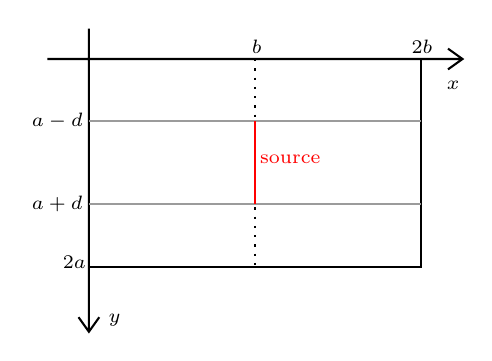
\begin{tikzpicture}[x=0.75pt,y=0.75pt,yscale=-1,xscale=1]
%uncomment if require: \path (0,300); %set diagram left start at 0, and has height of 300

%Straight Lines [id:da3480880018545507] 
\draw  [dash pattern={on 0.84pt off 2.51pt}]  (120,30) -- (120,130) ;
%Shape: Axis 2D [id:dp3637924149326488] 
\draw  (40,15.4) -- (40,161.4)(220,30) -- (20,30) (45,154.4) -- (40,161.4) -- (35,154.4) (213,25) -- (220,30) -- (213,35)  ;
%Shape: Rectangle [id:dp609433285561545] 
\draw   (40,30) -- (200,30) -- (200,130) -- (40,130) -- cycle ;
%Straight Lines [id:da15540762860028612] 
\draw [color={rgb, 255:red, 155; green, 155; blue, 155 }  ,draw opacity=1 ]   (40,60) -- (200,60) ;
%Straight Lines [id:da5236995862324196] 
\draw [color={rgb, 255:red, 155; green, 155; blue, 155 }  ,draw opacity=1 ]   (40,100) -- (200,100) ;
%Straight Lines [id:da00556491703537243] 
\draw [color={rgb, 255:red, 255; green, 0; blue, 0 }  ,draw opacity=1 ]   (120,60) -- (120,100) ;

% Text Node
\draw (211,39.4) node [anchor=north west][inner sep=0.75pt]  [font=\scriptsize]  {$x$};
% Text Node
\draw (48,151.4) node [anchor=north west][inner sep=0.75pt]  [font=\scriptsize]  {$y$};
% Text Node
\draw (194,19.4) node [anchor=north west][inner sep=0.75pt]  [font=\scriptsize]  {$2b$};
% Text Node
\draw (26,123.4) node [anchor=north west][inner sep=0.75pt]  [font=\scriptsize]  {$2a$};
% Text Node
\draw (117,19.4) node [anchor=north west][inner sep=0.75pt]  [font=\scriptsize]  {$b$};
% Text Node
\draw (11,54.4) node [anchor=north west][inner sep=0.75pt]  [font=\scriptsize]  {$a-d$};
% Text Node
\draw (11,94.4) node [anchor=north west][inner sep=0.75pt]  [font=\scriptsize]  {$a+d$};
% Text Node
\draw (121,75) node [anchor=north west][inner sep=0.75pt]  [font=\scriptsize,color={rgb, 255:red, 255; green, 0; blue, 0 }  ,opacity=1 ] [align=left] {source};


\end{tikzpicture}